\subsubsection{Résultats réduits et analyse - discussion}

\textbf{Méthode de réduction.} Pour chaque gaz, le déplacement $\Delta x = x_2 - x_1$ du curseur est calculé à partir des positions de deux maxima éloignés de $p$ maxima. Selon l'\refit{équation}{\eqref}{eq:vitesse-mesuree}, $\Delta x$ est proportionnel à $p/(2f)$ et la pente de la droite est la vitesse du son $v$. Le modèle ne comporte pas d'ordonnée à l'origine ($\Delta x = 0$ pour $p = 0$) : la régression linéaire est donc faite par la méthode des moindres carrés avec une droite passant par l'origine. L'incertitude sur la pente est déduite de la dispersion des points autour de la droite. La lecture d'une position est estimée à $\pm 0{,}5$ mm, soit $\pm 1$ mm sur $\Delta x$. L'incertitude sur $f$, mesurée au fréquencemètre, est négligeable.

Les valeurs théoriques sont calculées avec l'\refit{équation}{\eqref}{eq:vitesse-theorique}, avec $T$ la température relevée près du tube, incertaine de $\pm 0{,}5$ K, $\gamma$ incertain de $0{,}5\,\%$. Les constantes $R$ et $M$ sont considérées comme exactes.

Le \refit{Tableau}{\ref}{tab:recapitulatif-trombone} compare les vitesses mesurées et théoriques pour chaque gaz.

\begin{table}[H]
    \centering
    \small
    \begin{tabular}{lccccc}
        \toprule
        Gaz & $v_{\text{exp}}$ [m/s] & $\Delta v_{\text{exp}}/v_{\text{exp}}$ [\%] & $v_{\text{th}}$ [m/s] & $\Delta v_{\text{th}}/v_{\text{th}}$ [\%] & Écart [\%] \\
        \midrule
        Air         & $335{,}3 \pm 2{,}0$ & 0,6 & $345{,}3 \pm 0{,}9$ & 0,3 & 2,9 \\
        CO$_2$      & $272{,}2 \pm 1{,}5$ & 0,6 & $268{,}3 \pm 0{,}7$ & 0,3 & 1,5 \\
        \bottomrule
    \end{tabular}
    \caption{Tableau récapitulatif, résultats réduits, manipulation 2}
    \label{tab:recapitulatif-trombone}
\end{table}

\medskip

\textbf{Expérience - Air}\nopagebreak[4]

\begin{graphique}
    \centering
    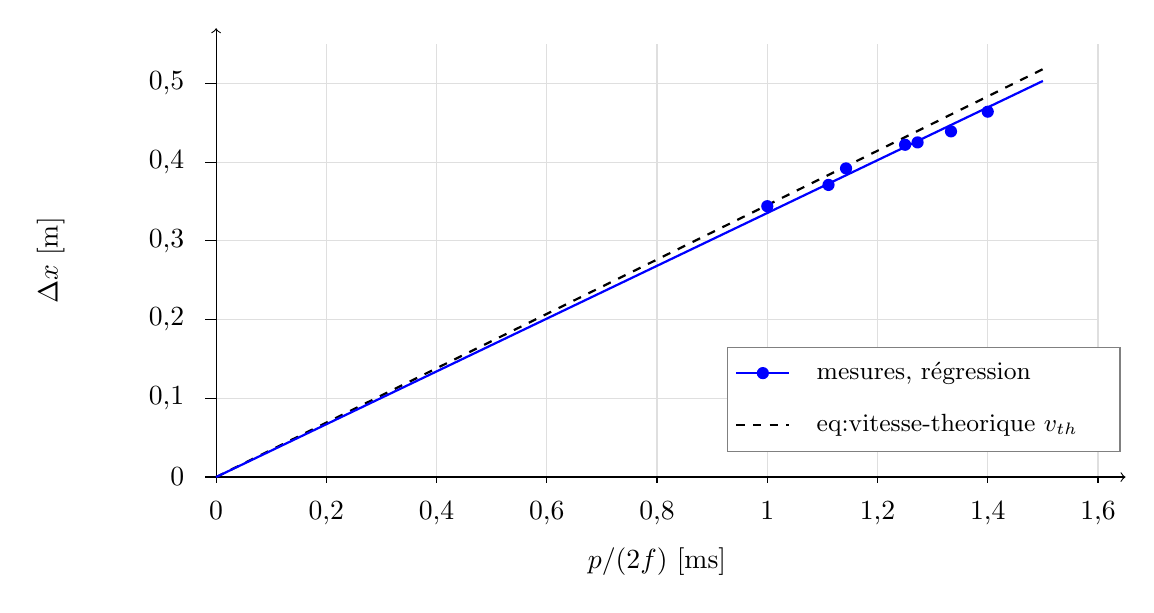
\begin{tikzpicture}[x=7cm,y=10cm]
        \foreach \x/\l in {0/0,0.2/0{,}2,0.4/0{,}4,0.6/0{,}6,0.8/0{,}8,1/1,1.2/1{,}2,1.4/1{,}4,1.6/1{,}6} {
            \draw[gray!25] (\x,0) -- (\x,0.55);
            \draw (\x,0) -- (\x,-0.008);
            \node[below=3pt] at (\x,-0.008) {\l};
        }
        \foreach \y/\l in {0/0,0.1/0{,}1,0.2/0{,}2,0.3/0{,}3,0.4/0{,}4,0.5/0{,}5} {
            \draw[gray!25] (0,\y) -- (1.6,\y);
            \draw (0,\y) -- (-0.02,\y);
            \node[left=4pt] at (-0.02,\y) {\l};
        }
        \draw[->] (0,0) -- (1.6500000000000001,0);
        \draw[->] (0,0) -- (0,0.5700000000000001);

        \draw[thick,dashed] (0,0) -- (1.5,0.5180);
        \draw[thick,blue] (0,0) -- (1.5,0.5030);
        \fill[blue] (1.0000,0.344) circle[radius=2.2pt];
        \fill[blue] (1.1429,0.392) circle[radius=2.2pt];
        \fill[blue] (1.2500,0.422) circle[radius=2.2pt];
        \fill[blue] (1.1111,0.371) circle[radius=2.2pt];
        \fill[blue] (1.4000,0.464) circle[radius=2.2pt];
        \fill[blue] (1.2727,0.425) circle[radius=2.2pt];
        \fill[blue] (1.3333,0.439) circle[radius=2.2pt];

        \draw[draw=gray,fill=white] (0.928,0.033) rectangle (1.640,0.165);
        \fill[blue] (0.992,0.132) circle[radius=2.2pt];
        \draw[thick,blue] (0.944,0.132) -- (1.040,0.132);
        \node[anchor=west,font=\small] at (1.072,0.132) {mesures, régression};
        \draw[thick,dashed] (0.944,0.066) -- (1.040,0.066);
        \node[anchor=west,font=\small] at (1.072,0.066) {\eqref{eq:vitesse-theorique} $v_{\text{th}}$};

        \node[below=22pt] at (0.80,0) {$p/(2f)$ [ms]};
        \node[rotate=90] at (-0.3,0.275) {$\Delta x$ [m]};
    \end{tikzpicture}
    \caption{Résultas réduits, expérience - Air}
    \label{fig:regression-air}
\end{graphique}

Le \refit{Graphique}{\ref}{fig:regression-air} montre $\Delta x$ en fonction de $p/(2f)$ pour l'air à $T = 297{,}1$ K. Les sept points, mesurés de $1\,500$ à $3\,000$ Hz, s'alignent le long d'une droite passant par l'origine, ce qui confirme qualitativement la \refit{relation}{\eqref}{eq:vitesse-mesuree} et le fait que la vitesse du son ne dépend pas de la fréquence dans ce domaine. La pente de la régression donne $v_{\text{exp}} = (335{,}3 \pm 2{,}0)$ m/s, soit une incertitude relative de $0{,}6\,\%$, alors que la valeur théorique est $v_{\text{th}} = (345{,}3 \pm 0{,}9)$ m/s. L'écart entre les deux valeurs est de $2{,}9\,\%$ ($10{,}0$ m/s), supérieur à l'incertitude expérimentale de $0{,}6\,\%$ ($2{,}0$ m/s) et à l'incertitude combinée de $0{,}6\,\%$ ($2{,}2$ m/s), la loi théorique est validée par cette mesure aux incertitudes expérimentales.
\medskip

\textbf{Expérience - CO$_2$}\nopagebreak[4]

\begin{graphique}
    \centering
    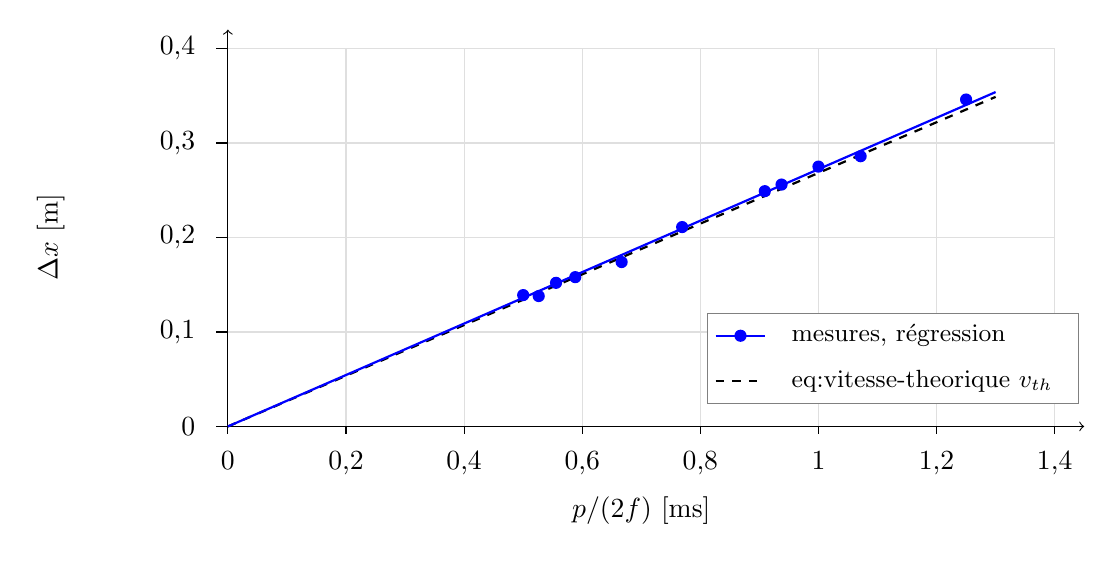
\begin{tikzpicture}[x=7.5cm,y=12cm]
        \foreach \x/\l in {0/0,0.2/0{,}2,0.4/0{,}4,0.6/0{,}6,0.8/0{,}8,1/1,1.2/1{,}2,1.4/1{,}4} {
            \draw[gray!25] (\x,0) -- (\x,0.4);
            \draw (\x,0) -- (\x,-0.008);
            \node[below=3pt] at (\x,-0.008) {\l};
        }
        \foreach \y/\l in {0/0,0.1/0{,}1,0.2/0{,}2,0.3/0{,}3,0.4/0{,}4} {
            \draw[gray!25] (0,\y) -- (1.4,\y);
            \draw (0,\y) -- (-0.02,\y);
            \node[left=4pt] at (-0.02,\y) {\l};
        }
        \draw[->] (0,0) -- (1.45,0);
        \draw[->] (0,0) -- (0,0.42000000000000004);

        \draw[thick,dashed] (0,0) -- (1.2999999999999998,0.3488);
        \draw[thick,blue] (0,0) -- (1.2999999999999998,0.3539);
        \fill[blue] (1.0000,0.275) circle[radius=2.2pt];
        \fill[blue] (0.9091,0.249) circle[radius=2.2pt];
        \fill[blue] (1.2500,0.346) circle[radius=2.2pt];
        \fill[blue] (0.7692,0.211) circle[radius=2.2pt];
        \fill[blue] (1.0714,0.286) circle[radius=2.2pt];
        \fill[blue] (0.6667,0.174) circle[radius=2.2pt];
        \fill[blue] (0.9375,0.256) circle[radius=2.2pt];
        \fill[blue] (0.5882,0.158) circle[radius=2.2pt];
        \fill[blue] (0.5556,0.152) circle[radius=2.2pt];
        \fill[blue] (0.5263,0.138) circle[radius=2.2pt];
        \fill[blue] (0.5000,0.139) circle[radius=2.2pt];

        \draw[draw=gray,fill=white] (0.812,0.024) rectangle (1.440,0.120);
        \fill[blue] (0.868,0.096) circle[radius=2.2pt];
        \draw[thick,blue] (0.826,0.096) -- (0.910,0.096);
        \node[anchor=west,font=\small] at (0.938,0.096) {mesures, régression};
        \draw[thick,dashed] (0.826,0.048) -- (0.910,0.048);
        \node[anchor=west,font=\small] at (0.938,0.048) {\eqref{eq:vitesse-theorique} $v_{\text{th}}$};

        \node[below=22pt] at (0.70,0) {$p/(2f)$ [ms]};
        \node[rotate=90] at (-0.3,0.200) {$\Delta x$ [m]};
    \end{tikzpicture}
    \caption{Résultas réduits, expérience - CO$_2$}
    \label{fig:regression-co2}
\end{graphique}

Le \refit{Graphique}{\ref}{fig:regression-co2} montre $\Delta x$ en fonction de $p/(2f)$ pour le CO$_2$ à $T = 296{,}3$ K. Les onze points, mesurés de $1\,000$ à $2\,000$ Hz, suivent aussi une droite passant par l'origine, avec $p = 2$ ou $3$ maxima, la vitesse du son est donc, qualitativement, indépendante de la fréquence. La pente donne $v_{\text{exp}} = (272{,}2 \pm 1{,}5)$ m/s, soit une incertitude relative de $0{,}6\,\%$, contre $v_{\text{th}} = (268{,}3 \pm 0{,}7)$ m/s. L'écart est de $1{,}5\,\%$ ($3{,}9$ m/s), supérieur à l'incertitude expérimentale de $0{,}6\,\%$ ($1{,}5$ m/s) et à l'incertitude combinée de $0{,}6\,\%$ ($1{,}7$ m/s), la loi théorique est validée aux incertitudes expérimentales.

Cet écart est faible et peut s'expliquer de plusieurs façons. Une présence résiduelle d'air dans le tube, aspiré de l'extérieur ou mal purgé, augmenterait la vitesse mesurée (la vitesse du son dans l'air est de $346$ m/s) et irait dans le sens de l'écart observé, de signe positif. Enfin, le petit nombre de maxima ($p = 2$ ou $3$) donne une incertitude relative sur $\Delta x$ de $0{,}3$ à $0{,}7\,\%$ par point, comme le montre la dispersion de la vitesse calculée point par point ($261$ à $278$ m/s).
